\documentclass[12pt,a4paper]{article}
\usepackage[utf8]{inputenc}

\usepackage{mathtools}
\usepackage{amsmath}
\usepackage{amssymb}
\usepackage{amsthm}
\usepackage{amssymb}
\usepackage{mathdots}
\usepackage[pdftex]{graphicx}
\usepackage{fancyhdr}
\usepackage[margin=1in]{geometry}
\usepackage{multicol}
\usepackage{bm}
\usepackage{listings}
\usepackage{xcolor}
\usepackage{pdfpages}
\usepackage{algpseudocode}
\usepackage{tikz}
\usepackage{enumitem}
\usepackage[T1]{fontenc}
\usepackage{inconsolata}
\usepackage{framed}
\usepackage{wasysym}
\usepackage[thinlines]{easytable}
\usepackage{hyperref}
\usepackage{minted}
\usemintedstyle{perldoc}
\hypersetup{
    colorlinks=true,
    linkcolor=blue,
    filecolor=magenta,      
    urlcolor=blue,
}
\definecolor{codegreen}{rgb}{0,0.6,0}
\definecolor{codegray}{rgb}{0.5,0.5,0.5}
\definecolor{codepurple}{rgb}{0.58,0,0.82}
\definecolor{backcolour}{rgb}{0.95,0.95,0.92}
\lstdefinestyle{mystyle}{
    backgroundcolor=\color{backcolour},   
    commentstyle=\color{codegreen},
    keywordstyle=\color{magenta},
    numberstyle=\tiny\color{codegray},
    stringstyle=\color{codepurple},
    basicstyle=\ttfamily,
    breakatwhitespace=false,         
    breaklines=true,                 
    captionpos=b,                    
    keepspaces=true,                 
    numbers=left,                    
    numbersep=5pt,                  
    showspaces=false,                
    showstringspaces=false,
    showtabs=false,                  
    tabsize=4
}
\lstset{style=mystyle}
\newcommand\numberthis{\addtocounter{equation}{1}\tag{\theequation}}
\newcommand{\rightqed}{
\begin{flushright}
$\blacksquare$
\end{flushright}
}
\newcommand{\solution}{\noindent\textbf{Solution:}\\\indent}
\usepackage{graphics}
\usepackage{subfig}
\graphicspath{ {./images/} }

\title{CSCI 6690 Spectral Graph Theory Homework 6\\Comparing Graphs}
\author{Kushajveer Singh}
\date{}

\begin{document}
\maketitle

% Start problem 1
\subsection*{Problem 1(1)}
\textit{
    Prove $A \succeq B$ and $B \succeq C \implies A \succeq C$
}

\solution
Consider $\vec{v} \in \mathbb{R}^n$. By definition we have,
\begin{align}
    A \succeq B &\implies \langle \vec{v}, \vec{v} \rangle_A \geq \langle \vec{v}, \vec{v} \rangle_B \label{eq:1_1} \\
    B \succeq C &\implies \langle \vec{v}, \vec{v} \rangle_B \geq \langle \vec{v}, \vec{v} \rangle_C \label{eq:1_2}
\end{align}

Comparing \eqref{eq:1_1} and \eqref{eq:1_2} we get
\begin{align}
    \langle \vec{v}, \vec{v} \rangle_A &\geq \langle \vec{v}, \vec{v} \rangle_C \\
    \implies A &\succeq C
\end{align}
\rightqed

\subsection*{Problem 1(2)}
\textit{
    Prove $A \succeq B \implies A + C \succeq B + C$
}

\solution
Consider $\vec{v} \in \mathbb{R}^n$. By definition we have,
\begin{align*}
    \langle \vec{v}, \vec{v} \rangle_{A+C} &= \langle \vec{v}, (A+C)\vec{v} \rangle \\
    &= \langle \vec{v}, A\vec{v} \rangle + \langle \vec{v}, C\vec{v} \rangle \numberthis \label{eq:1_3} \\
    \langle \vec{v}, \vec{v} \rangle_{B+C} &= \langle \vec{v}, (B+C)\vec{v} \rangle \\
    &= \langle \vec{v}, B\vec{v} \rangle + \langle \vec{v}, C\vec{v} \rangle \numberthis \label{eq:1_4} \\
\end{align*}

Comparing \eqref{eq:1_3} and \eqref{eq:1_4}, we know $\langle \vec{v}, A\vec{v} \rangle \geq \langle \vec{v}, B\vec{v} \rangle$ (as $A\succeq B$), which implies
\begin{align*}
    \langle \vec{v}, \vec{v} \rangle_{A+C} &\geq \langle \vec{v}, \vec{v} \rangle_{B+C} \\
    \implies A + C &\succeq B + C \numberthis
\end{align*}
\rightqed

\newpage
\subsection*{Problem 2}
\textit{
    Prove that $T_d$ is isomorphic to $\mathcal{T}_d$
}

\solution
To help with visualization figure \ref{fig:2_1} shows $T_3$ on left and $\mathcal{T}_3$ on right.

\begin{figure}[H]
    \centering
    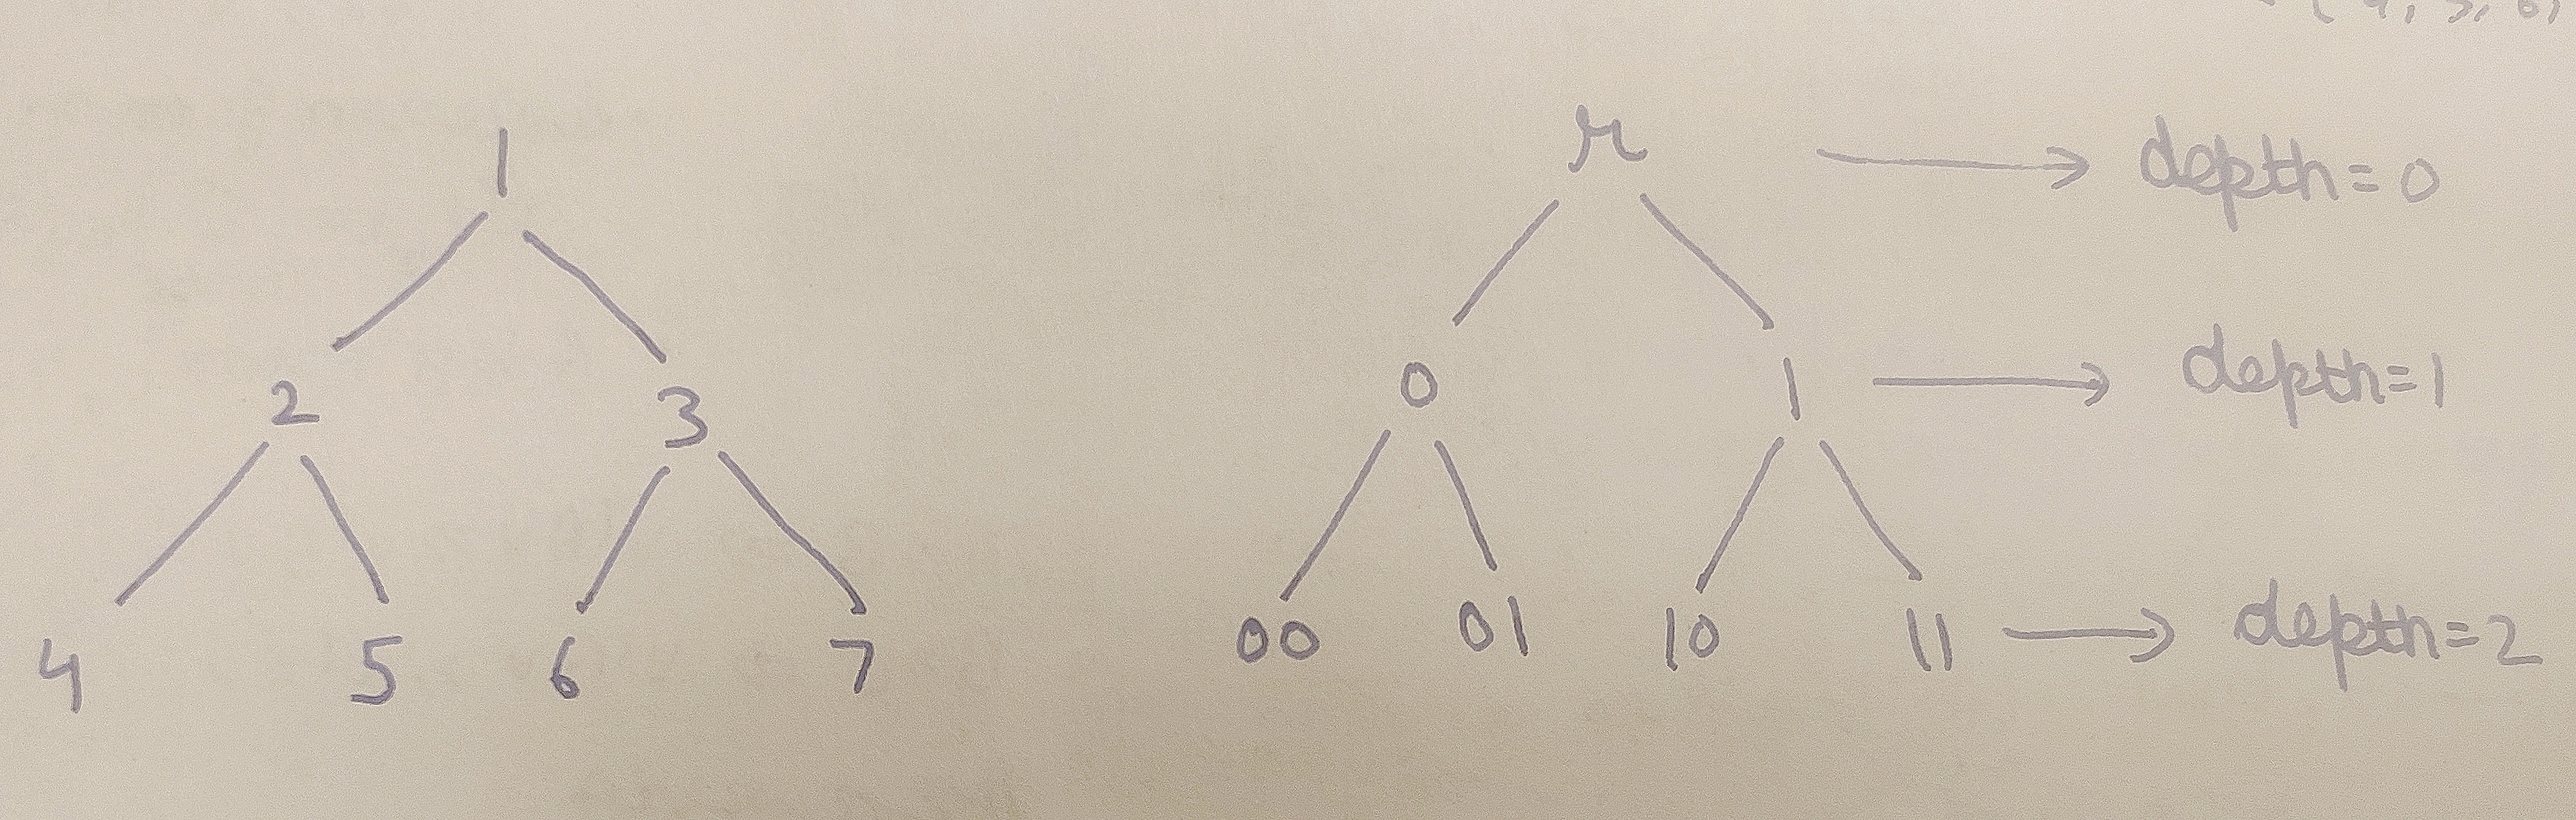
\includegraphics[width=\textwidth]{prob_2.jpg}
    \caption{Shows $T_3$ on left and $\mathcal{T}_3$ on right}
    \label{fig:2_1}
\end{figure}

Consider a function $f$ which maps vertices from $T_d$ to $\mathcal{T}_d$. The function $f$ can be defined as mapping vertex $i$ in $T_d$ to the binary representation of $i$ and considering considering $floor(log_2(i))$ digits from the left of the representation (i.e. remove the most significant bit from the representation). For base case $i=1$, the function has an exception where it maps $f(1) = r$. For example, $i=6$ has a binary representation of $110$ and it is mapped to $10$.

At depth = d, the function outputs a $2^d$ unique strings with number of digits equal to $d$, which means $f$ produces a one-to-one mapping from vertices in $T_d$ to vertices in $\mathcal{T}_d$.

In $T_d$, every vertex $i$ is connected to $2i$ and $2i+1$. If $b_1b_2\hdots b_d$ is the binary representation outputted by $f(i)$, then the binary representation of $2*i$ and $2*i+1$ is given as $b_1b_2\hdots b_d0$ and $b_1b_2\hdots b_d1$ respectively. And this is the same edge mapping in $\mathcal{T}_d$. Therefore we have shown that the function $f$ induces a bijection between the edges of $T_d$ and edges of $\mathcal{T}_d$.

Consider a function $g$ which maps vertices from $\mathcal{T}_d$ to $T_d$. The function $g$ can be defined as mapping string $x$ in $\mathcal{T}_d$ to ($2^{length\ of\ x} + decimal\_repr(x)$). For base case $x=r$, the function has an exception where it maps $g(r) = 1$. For example, $x=10$ has length = 2 and decimal representation = 2. So $g(10) = 2^2 + 2 = 6$.

At depth = d, the function outputs values from $2^d$ to $2^{d+1}-1$, which means $g$ produces a one-to-one mapping from strings in $\mathcal{T}_d$ to vertices in $T_d$.

In $\mathcal{T}_d$, every string $x$ has $x0$ and $x1$ as children. Let length of $x$ be $d$, then $g(x) = 2^d + y$, where y is decimal representation of $x$. Now,
\begin{align*}
    g(x0) &= 2^{d+1} + 2*y + 0 \\
          &= 2(2^d + y) \\
          &= 2g(x) \numberthis \label{eq:2_1}\\
    g(x1) &= 2^{d+1} + 2*y + 1 \\
          &= 2(2^d + y) + 1 \\
          &= 2g(x) + 1 \numberthis \label{eq:2_2}
\end{align*}

\eqref{eq:2_1} and \eqref{eq:2_2} are the same edge mapping as $T_d$. Therefore we have shown that the function $g$ induces a bijection between the edges of $\mathcal{T}_d$ and edges of $T_d$.

We found $f$ to be a bijective mapping from vertices of $T_d$ to $\mathcal{T}_d$ and $g$ to be a bijective mapping from vertices of $\mathcal{T}_d$ to $T_d$. It is also shown that these mapping induce a bijection between the edges of the graphs also.
\rightqed


\newpage
\subsection*{Problem 3}
\textit{
    Prove $\|\vec{v}\| \leq \|\vec{v} + t\vec{1}\|$
}

\solution
Suppose $\vec{v} \in \mathbb{R}^n$. Given $\langle \vec{v}, \vec{1} \rangle = 0$, which implies
\begin{equation}
    v_1 + v_2 + \hdots + v_n = 0 \label{eq:3_1}
\end{equation}

We need to prove,
\begin{align}
    \|\vec{v}\| &\leq \|\vec{v} + t\vec{1}\| \\
    \sqrt{v_1^2 + v_2^2 + \hdots + v_n^2} &\leq \sqrt{(v_1+t)^2 + (v_2+t)^2 + \hdots + (v_n+t)^2} \label{eq:3_2} \\
    v_1^2 + v_2^2 + \hdots + v_n^2 &\leq (v_1+t)^2 + (v_2+t)^2 + \hdots + (v_n+t)^2 \label{eq:3_3} \\
    v_1^2 + v_2^2 + \hdots + v_n^2 &\leq v_1^2 + v_2^2 + \hdots + v_n^2 + nt^2 + 2t(v_1+v_2+ \hdots + v_n) \\
    0 &\leq nt^2 + 2t(v_1 + v_2 + \hdots + v_n) \label{eq:3_5} \\
    0 &\leq nt^2 \label{eq:3_6}
\end{align}

In \eqref{eq:3_2}, $\|.\|$ notation is expanded to refer to L2-norm of a vector.\\
\indent In \eqref{eq:3_3}, square root can be removed without loss of generality (by squaring both sides)
\indent In \eqref{eq:3_5}, the $\sum_{i=1}^nv_i^2$ term gets cancelled on both sides of equation \\
\indent In \eqref{eq:3_6}, we use the result from \eqref{eq:3_1} \\

We observe that $nt^2 \geq 0$ is valid for all non-negative values.
\rightqed
\end{document}
